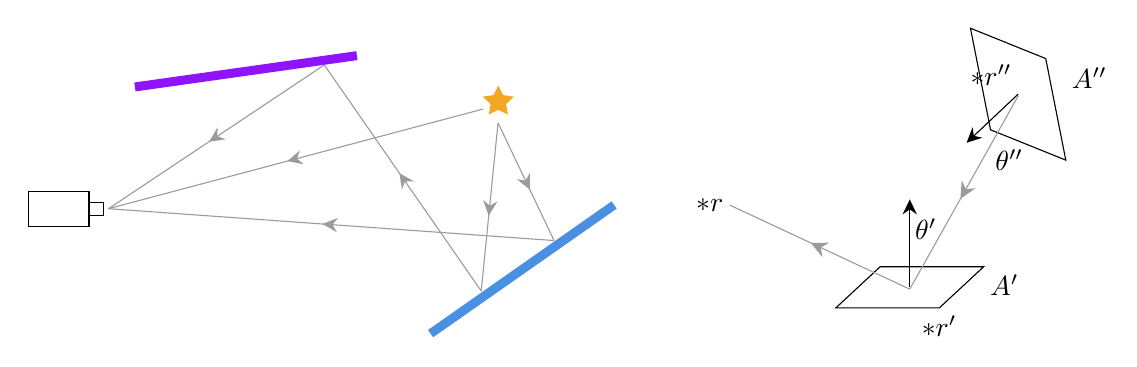
\begin{tikzpicture}[x=0.75pt,y=0.75pt,yscale=-0.9,xscale=0.9]
    %uncomment if require: \path (0,300); %set diagram left start at 0, and has height of 300
    
    %Shape: Rectangle [id:dp5200245791087557] 
    \draw   (25.67,111.67) -- (58.22,111.67) -- (58.22,130.27) -- (25.67,130.27) -- cycle ;
    %Shape: Rectangle [id:dp7846538223375579] 
    \draw   (58.25,117.64) -- (66.14,117.64) -- (66.14,124.3) -- (58.25,124.3) -- cycle ;
    
    %Shape: Star [id:dp5332215332179218] 
    \draw  [draw opacity=0][fill={rgb, 255:red, 245; green, 166; blue, 35 }  ,fill opacity=1 ] (277.34,54.94) -- (279.9,60.08) -- (285.65,60.9) -- (281.49,64.9) -- (282.47,70.55) -- (277.34,67.88) -- (272.2,70.55) -- (273.18,64.9) -- (269.03,60.9) -- (274.77,60.08) -- cycle ;
    %Shape: Rectangle [id:dp16700693443291525] 
    \draw  [draw opacity=0][fill={rgb, 255:red, 74; green, 144; blue, 226 }  ,fill opacity=1 ] (239.69,185.8) -- (337.96,116.94) -- (340.71,120.87) -- (242.44,189.73) -- cycle ;
    %Straight Lines [id:da4511556653356976] 
    \draw [color={rgb, 255:red, 155; green, 155; blue, 155 }  ,draw opacity=1 ]   (68.64,120.89) -- (269.2,67.55) ;
    \draw [shift={(164.38,95.43)}, rotate = 345.11] [fill={rgb, 255:red, 155; green, 155; blue, 155 }  ,fill opacity=1 ][line width=0.08]  [draw opacity=0] (8.04,-3.86) -- (0,0) -- (8.04,3.86) -- (5.34,0) -- cycle    ;
    %Straight Lines [id:da4022715793961895] 
    \draw [color={rgb, 255:red, 155; green, 155; blue, 155 }  ,draw opacity=1 ]   (307.17,137.94) -- (277.17,74.94) ;
    \draw [shift={(294.19,110.68)}, rotate = 244.54] [fill={rgb, 255:red, 155; green, 155; blue, 155 }  ,fill opacity=1 ][line width=0.08]  [draw opacity=0] (8.04,-3.86) -- (0,0) -- (8.04,3.86) -- (5.34,0) -- cycle    ;
    %Straight Lines [id:da16168522569161548] 
    \draw [color={rgb, 255:red, 155; green, 155; blue, 155 }  ,draw opacity=1 ]   (68.64,120.89) -- (307.17,137.94) ;
    \draw [shift={(183.22,129.08)}, rotate = 4.09] [fill={rgb, 255:red, 155; green, 155; blue, 155 }  ,fill opacity=1 ][line width=0.08]  [draw opacity=0] (8.04,-3.86) -- (0,0) -- (8.04,3.86) -- (5.34,0) -- cycle    ;
    %Shape: Rectangle [id:dp7490783622220103] 
    \draw  [draw opacity=0][fill={rgb, 255:red, 144; green, 19; blue, 254 }  ,fill opacity=1 ] (82.45,53.34) -- (201.28,36.58) -- (201.95,41.33) -- (83.12,58.1) -- cycle ;
    %Straight Lines [id:da05078643662124227] 
    \draw [color={rgb, 255:red, 155; green, 155; blue, 155 }  ,draw opacity=1 ]   (268.17,164.94) -- (277.17,74.94) ;
    \draw [shift={(272.2,124.61)}, rotate = 275.71] [fill={rgb, 255:red, 155; green, 155; blue, 155 }  ,fill opacity=1 ][line width=0.08]  [draw opacity=0] (8.04,-3.86) -- (0,0) -- (8.04,3.86) -- (5.34,0) -- cycle    ;
    %Straight Lines [id:da607422690270008] 
    \draw [color={rgb, 255:red, 155; green, 155; blue, 155 }  ,draw opacity=1 ]   (268.17,164.94) -- (184.17,43.94) ;
    \draw [shift={(224.34,101.81)}, rotate = 55.23] [fill={rgb, 255:red, 155; green, 155; blue, 155 }  ,fill opacity=1 ][line width=0.08]  [draw opacity=0] (8.04,-3.86) -- (0,0) -- (8.04,3.86) -- (5.34,0) -- cycle    ;
    %Straight Lines [id:da08130692168711917] 
    \draw [color={rgb, 255:red, 155; green, 155; blue, 155 }  ,draw opacity=1 ]   (68.64,120.89) -- (184.17,43.94) ;
    \draw [shift={(122.49,85.02)}, rotate = 326.33] [fill={rgb, 255:red, 155; green, 155; blue, 155 }  ,fill opacity=1 ][line width=0.08]  [draw opacity=0] (8.04,-3.86) -- (0,0) -- (8.04,3.86) -- (5.34,0) -- cycle    ;
    %Shape: Parallelogram [id:dp6430851072923569] 
    \draw   (481.75,151.94) -- (537.17,151.94) -- (513.42,174) -- (458,174) -- cycle ;
    %Shape: Parallelogram [id:dp8807704832359311] 
    \draw   (540.83,78.64) -- (530.09,24.28) -- (570.37,40.52) -- (581.11,94.89) -- cycle ;
    %Straight Lines [id:da5099223782326536] 
    \draw    (497.58,118.94) -- (497.58,162.97) ;
    \draw [shift={(497.58,115.94)}, rotate = 90] [fill={rgb, 255:red, 0; green, 0; blue, 0 }  ][line width=0.08]  [draw opacity=0] (8.04,-3.86) -- (0,0) -- (8.04,3.86) -- (5.34,0) -- cycle    ;
    %Straight Lines [id:da5428576192715366] 
    \draw    (530.2,83.52) -- (555.6,59.58) ;
    \draw [shift={(528.01,85.58)}, rotate = 316.69] [fill={rgb, 255:red, 0; green, 0; blue, 0 }  ][line width=0.08]  [draw opacity=0] (8.04,-3.86) -- (0,0) -- (8.04,3.86) -- (5.34,0) -- cycle    ;
    %Straight Lines [id:da21616936796564357] 
    \draw [color={rgb, 255:red, 155; green, 155; blue, 155 }  ,draw opacity=1 ]   (555.6,60.58) -- (497.58,163.97) ;
    \draw [shift={(524.73,115.59)}, rotate = 299.3] [fill={rgb, 255:red, 155; green, 155; blue, 155 }  ,fill opacity=1 ][line width=0.08]  [draw opacity=0] (8.93,-4.29) -- (0,0) -- (8.93,4.29) -- (5.93,0) -- cycle    ;
    %Straight Lines [id:da476245189923] 
    \draw [color={rgb, 255:red, 155; green, 155; blue, 155 }  ,draw opacity=1 ]   (401.17,118.94) -- (497.58,163.97) ;
    \draw [shift={(444.57,139.21)}, rotate = 25.03] [fill={rgb, 255:red, 155; green, 155; blue, 155 }  ,fill opacity=1 ][line width=0.08]  [draw opacity=0] (8.93,-4.29) -- (0,0) -- (8.93,4.29) -- (5.93,0) -- cycle    ;
    
    % Text Node
    \draw (499,125) node [anchor=north west][inner sep=0.75pt]    {$\theta '$};
    % Text Node
    \draw (542,88) node [anchor=north west][inner sep=0.75pt]    {$\theta ''$};
    % Text Node
    \draw (583,44) node [anchor=north west][inner sep=0.75pt]    {$\dd A''$};
    % Text Node
    \draw (539.17,154.94) node [anchor=north west][inner sep=0.75pt]    {$\dd A'$};
    % Text Node
    \draw (553.6,56.58) node [anchor=south east] [inner sep=0.75pt]    {$\vb*{r}''$};
    % Text Node
    \draw (513.42,177) node [anchor=north] [inner sep=0.75pt]    {$\vb*{r}'$};
    % Text Node
    \draw (399.17,118.94) node [anchor=east] [inner sep=0.75pt]    {$\vb*{r}$};
    
    
    \end{tikzpicture}
    